\documentclass[../../dissertation.tex]{subfiles}
\begin{document}

Consider the example of a quantum walker on a discretely numbered cycle. It was seen that the evolution operator associated with such a system is, as was defined in equation \ref{eq:coinedUnmarkedOperator}
\begin{equation}
	   U = S(C\otimes I), 
           \label{eq:coinedUnmarkedOperatorQiskit}
\end{equation}
%TODO: Decidir se menciono as equacoes do shift e da coin.
where $S$ is a shift operator, defined in equation \ref{eq:coinedShiftOperator} as 
\begin{equation}
          S = \ket{0}\bra{0} \otimes \sum_{x=-\infty}^{x=\infty} \ket{x+1}\bra{x} + \ket{1}\bra{1}\otimes \sum_{x=-\infty}^{x=\infty} \ket{x-1}\bra{x},
\end{equation} 
that increments or decrements the position of the walker according to the coin operator $C$.\par
%TODO: Reescrever prox paragrafo.
Previously, this system was simulated in Python by implenting it's equations. Now, the focus is to study a quantum circuit based on the work presented by \cite{douglaswang07}. This approach relies on multi-controlled CNOT gates in order to shift the state of the walker by $+1$ or $-1$, each with a probability associated with the chosen coin, as can be seen in figure \ref{fig:douglasWangShift}. 

%TODO: Decidir se ficam 3 pontos verticais.
%TODO: Substituir todas as minipages por subfigures.
\begin{figure}[!htb]
	\centering
	\begin{subfigure}[t]{0.40\textwidth}
        \[ \Qcircuit @C=1em @R=.7em {& \targ    & \qw      & \qw      & \qw      & \qw \\
        			  & 	     & 	        &          &          &  . \\
        			  & 	     & 	        &          &          &  . \\
        			  & 	     & 	        &          &          &  . \\
        			  & \ctrl{-4} & \targ   & \qw      & \qw      & \qw \\
        			  & \ctrl{-1} & \ctrl{-1} & \targ    & \qw      & \qw\\ 
        			  & \ctrl{-1} & \ctrl{-1} & \ctrl{-1} & \qw      & \qw
			  } \]
	\caption{Douglas wang increment}
	\label{fig:coinedIncrement}
	\end{subfigure}
	\begin{subfigure}[t]{0.40\textwidth}
        \[ \Qcircuit @C=1em @R=.7em {& \targ    & \qw      & \qw      & \qw      & \qw \\
        			  & 	     & 	        &          &          &  . \\
        			  & 	     & 	        &          &          &  . \\
        			  & 	     & 	        &          &          &  . \\
        			  & \ctrlo{-4} & \targ   & \qw      & \qw      & \qw \\
        			  & \ctrlo{-1} & \ctrlo{-1} & \targ    & \qw      & \qw\\ 
        			  & \ctrlo{-1} & \ctrlo{-1} & \ctrlo{-1} & \qw      & \qw
			  } \]
	\centering
	\caption{Douglas wang Decrement}
	\label{fig:coinedDecrement}
	\end{subfigure}
	\caption{Douglas wang shift operator}
	\label{fig:douglasWangShift}
\end{figure}

%TODO: Melhorar o paragrafo seguinte
The generalized CNOT gates act on the node states as a cyclic permutator, where each node is mapped to an adjacent state. This can be seen as the walker moving left or right, in the uni-dimensional graph example.\par

%TODO: Descobrir como separar a moeda do resto do circuito. Adicionar node e subnode?
%TODO: Fazer um circuito para N=3 ou N=4 e por os resultados da simulacao com esse numero. 
%TODO: Resize da figura?
\begin{figure}[!h]
	\[ \Qcircuit @C=1em @R=0em { &\qw & \multigate{4}{incr} &  \multigate{4}{decr} & \qw \\
				     &\qw & \ghost{incr} & \ghost{decr} & \qw \\
               			     &\qw & \ghost{incr} & \ghost{decr} & \qw \\
            			     &\qw & \ghost{incr} & \ghost{decr} & \qw \\
            			     &\qw & \ghost{incr} & \ghost{decr} & \qw \\ 
				     &    &              &              &     \\
				     &    &              &              &     \\
				     &    &              &              &     \\
				     &\gate{H} & \ctrl{-2} & \ctrlo{-2} & \qw 
		          } \]
	\centering
	\caption{Douglas wang coined quantum walk circuit}
	\label{fig:coinedCircuit}
\end{figure}

The coin operator will simply be a Hadamard gate acting on a single qubit. For a graph with $16$ nodes, for example, $4$ qubits are required to encode each node and an extra qubit for the coin. The circuit will then be as shown in figure \ref{fig:coinedCircuit}. Note that this circuit limits the number of graph nodes to powers of $2$, and an arbitrary implementation of $2^n$ nodes requires $n+1$ qubits.
%TODO: Decidir como falar sobre como implementar nos que nao sao potencias de 2. Deverei mencionar a figura do artigo do doulgas wang?
%TODO: Descobrir uma source diferente para o gray code ordering. Nielsen chuang.
However, it is possible to have any number of nodes, given that the proper correction is made as can be seen in \cite{douglaswang07}. The method used was \textit{Gray Code Ordering} proposed by \cite{alexslepoy06}, whereby a certain arrangement of CNOT gates results in control states only differing by a single bit.\par
In order to run this circuit on a real quantum computer, using Qiskit, one must first find a way of creating generalized CNOT gates, since it is not available in the base package. One approach to this problem is to decompose an arbitrarily controlled CNOT gate into elementary gates, as was done by \cite{barenco95}.
%TODO: Explicar a decomposicao da cnot? Ver a dissertacao.


\begin{figure}[!h]
	\centering
	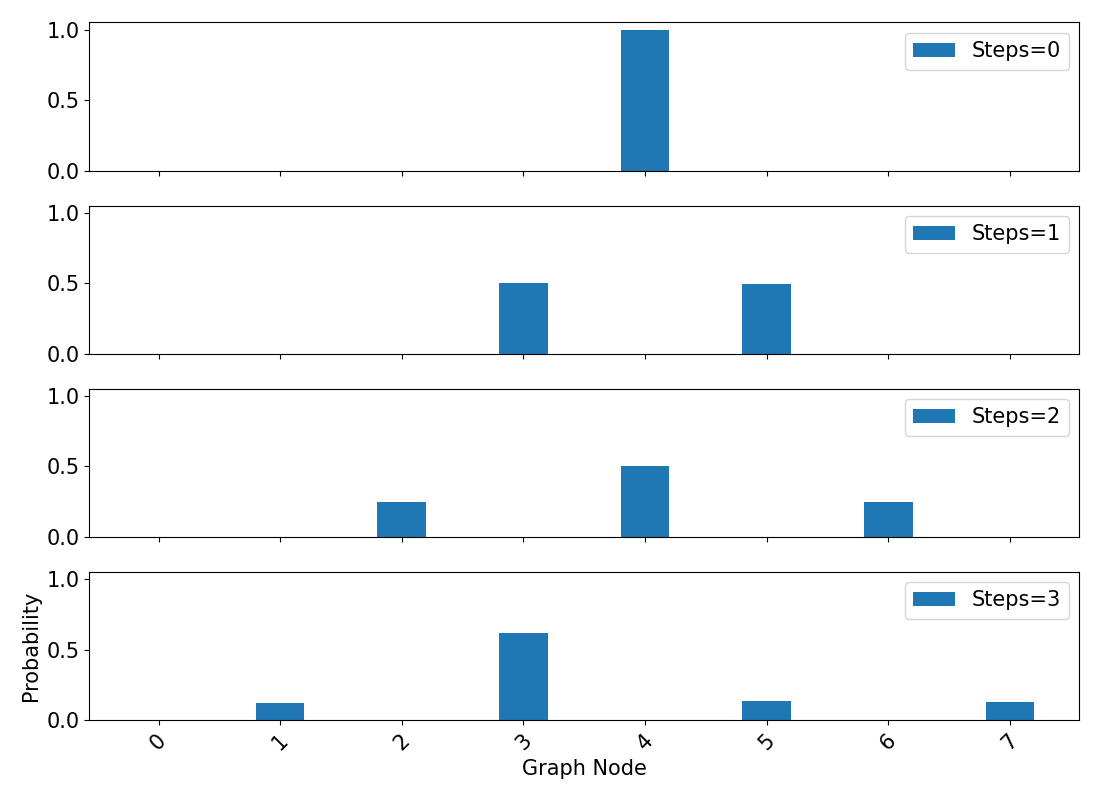
\includegraphics[scale=0.40]{img/Qiskit/CoinedQuantumWalk/CoinedQW_N3_S0123.png}
	\caption{Probability distribution for the staggered quantum walk on a line after 50 steps, with initial condition $\ket{\Psi(0)}=\frac{\ket{0}+\ket{1}}{\sqrt{2}}$, for multiple angles.} 
	\label{fig:fig5}
\end{figure}

\end{document}
